\documentclass[pdf]{beamer}
\mode<presentation>{}

\usetheme{Frankfurt}
\usepackage{listings}
\usepackage{color}
\usepackage{amsmath}


\usefonttheme[onlymath]{serif}

%% preamble
\title[Random Forests]{CART, Bagging, and Random Forests}

\author{}
\date{}

\begin{document}

%% title frame
\begin{frame}
\titlepage
\end{frame}



\begin{frame}<beamer>{Table of Contents}
	\tableofcontents[currentsection, 
				 currentsubsection, 
				 sectionstyle=show, 
				 subsectionstyle=show]
\end{frame}


\section{Introduction}
	\subsection{Trees}
		\begin{frame}{Species of Tree-Based Models}
			\begin{enumerate}
				\item{ID3}
				\item{C4.5}
				\item{C5.0}
				\item{CART}
			\end{enumerate}
		\end{frame}
			
	
	\subsection{Example}	
		
		\begin{frame}{Titanic Example}
			\begin{enumerate}
				\item{Titantic data}
				\item{Kaggle competition}
				\item{Predicting survival (2-class problem)}
				\item{Using demographic and other variables}
			\end{enumerate}
		\end{frame}
		
		
		
		\begin{frame}{Titanic Data}
		\begin{table}
		\begin{tabular}{l c c c c c c}
			\hline
			survived & age & sex & pclass & fare & sibsp & parch \\
			\hline
			1 	& 29.00 	& female	& 1	& 211.34	& 0	& 0 \\
			1 	& 0.92 	& male	& 1	& 151.55	& 1	& 2 \\
			0	& 2.00	& female	& 1	& 151.55	& 1	& 2 \\
			0 	& 30.00 	& male	& 1	& 151.55	& 1	& 2 \\
			0	& 25.00	& female	& 1	& 151.55	& 1	& 2 \\
			1 	& 48.00 	& male	& 1	& 151.55	& 0	& 0 \\
			1	& 63.00	& female	& 1	& 26.55	& 1	& 0 \\
			0	& 39.00	& male	& 1	& 0.00	& 0	& 0 \\
			1 	& 53.00 	& female	& 1	& 51.48	& 2	& 0 \\
			\hline
		\end{tabular}
		\end{table}
		\end{frame}
		
		
		\begin{frame}{Titanic Survial}
			\begin{figure}
		%		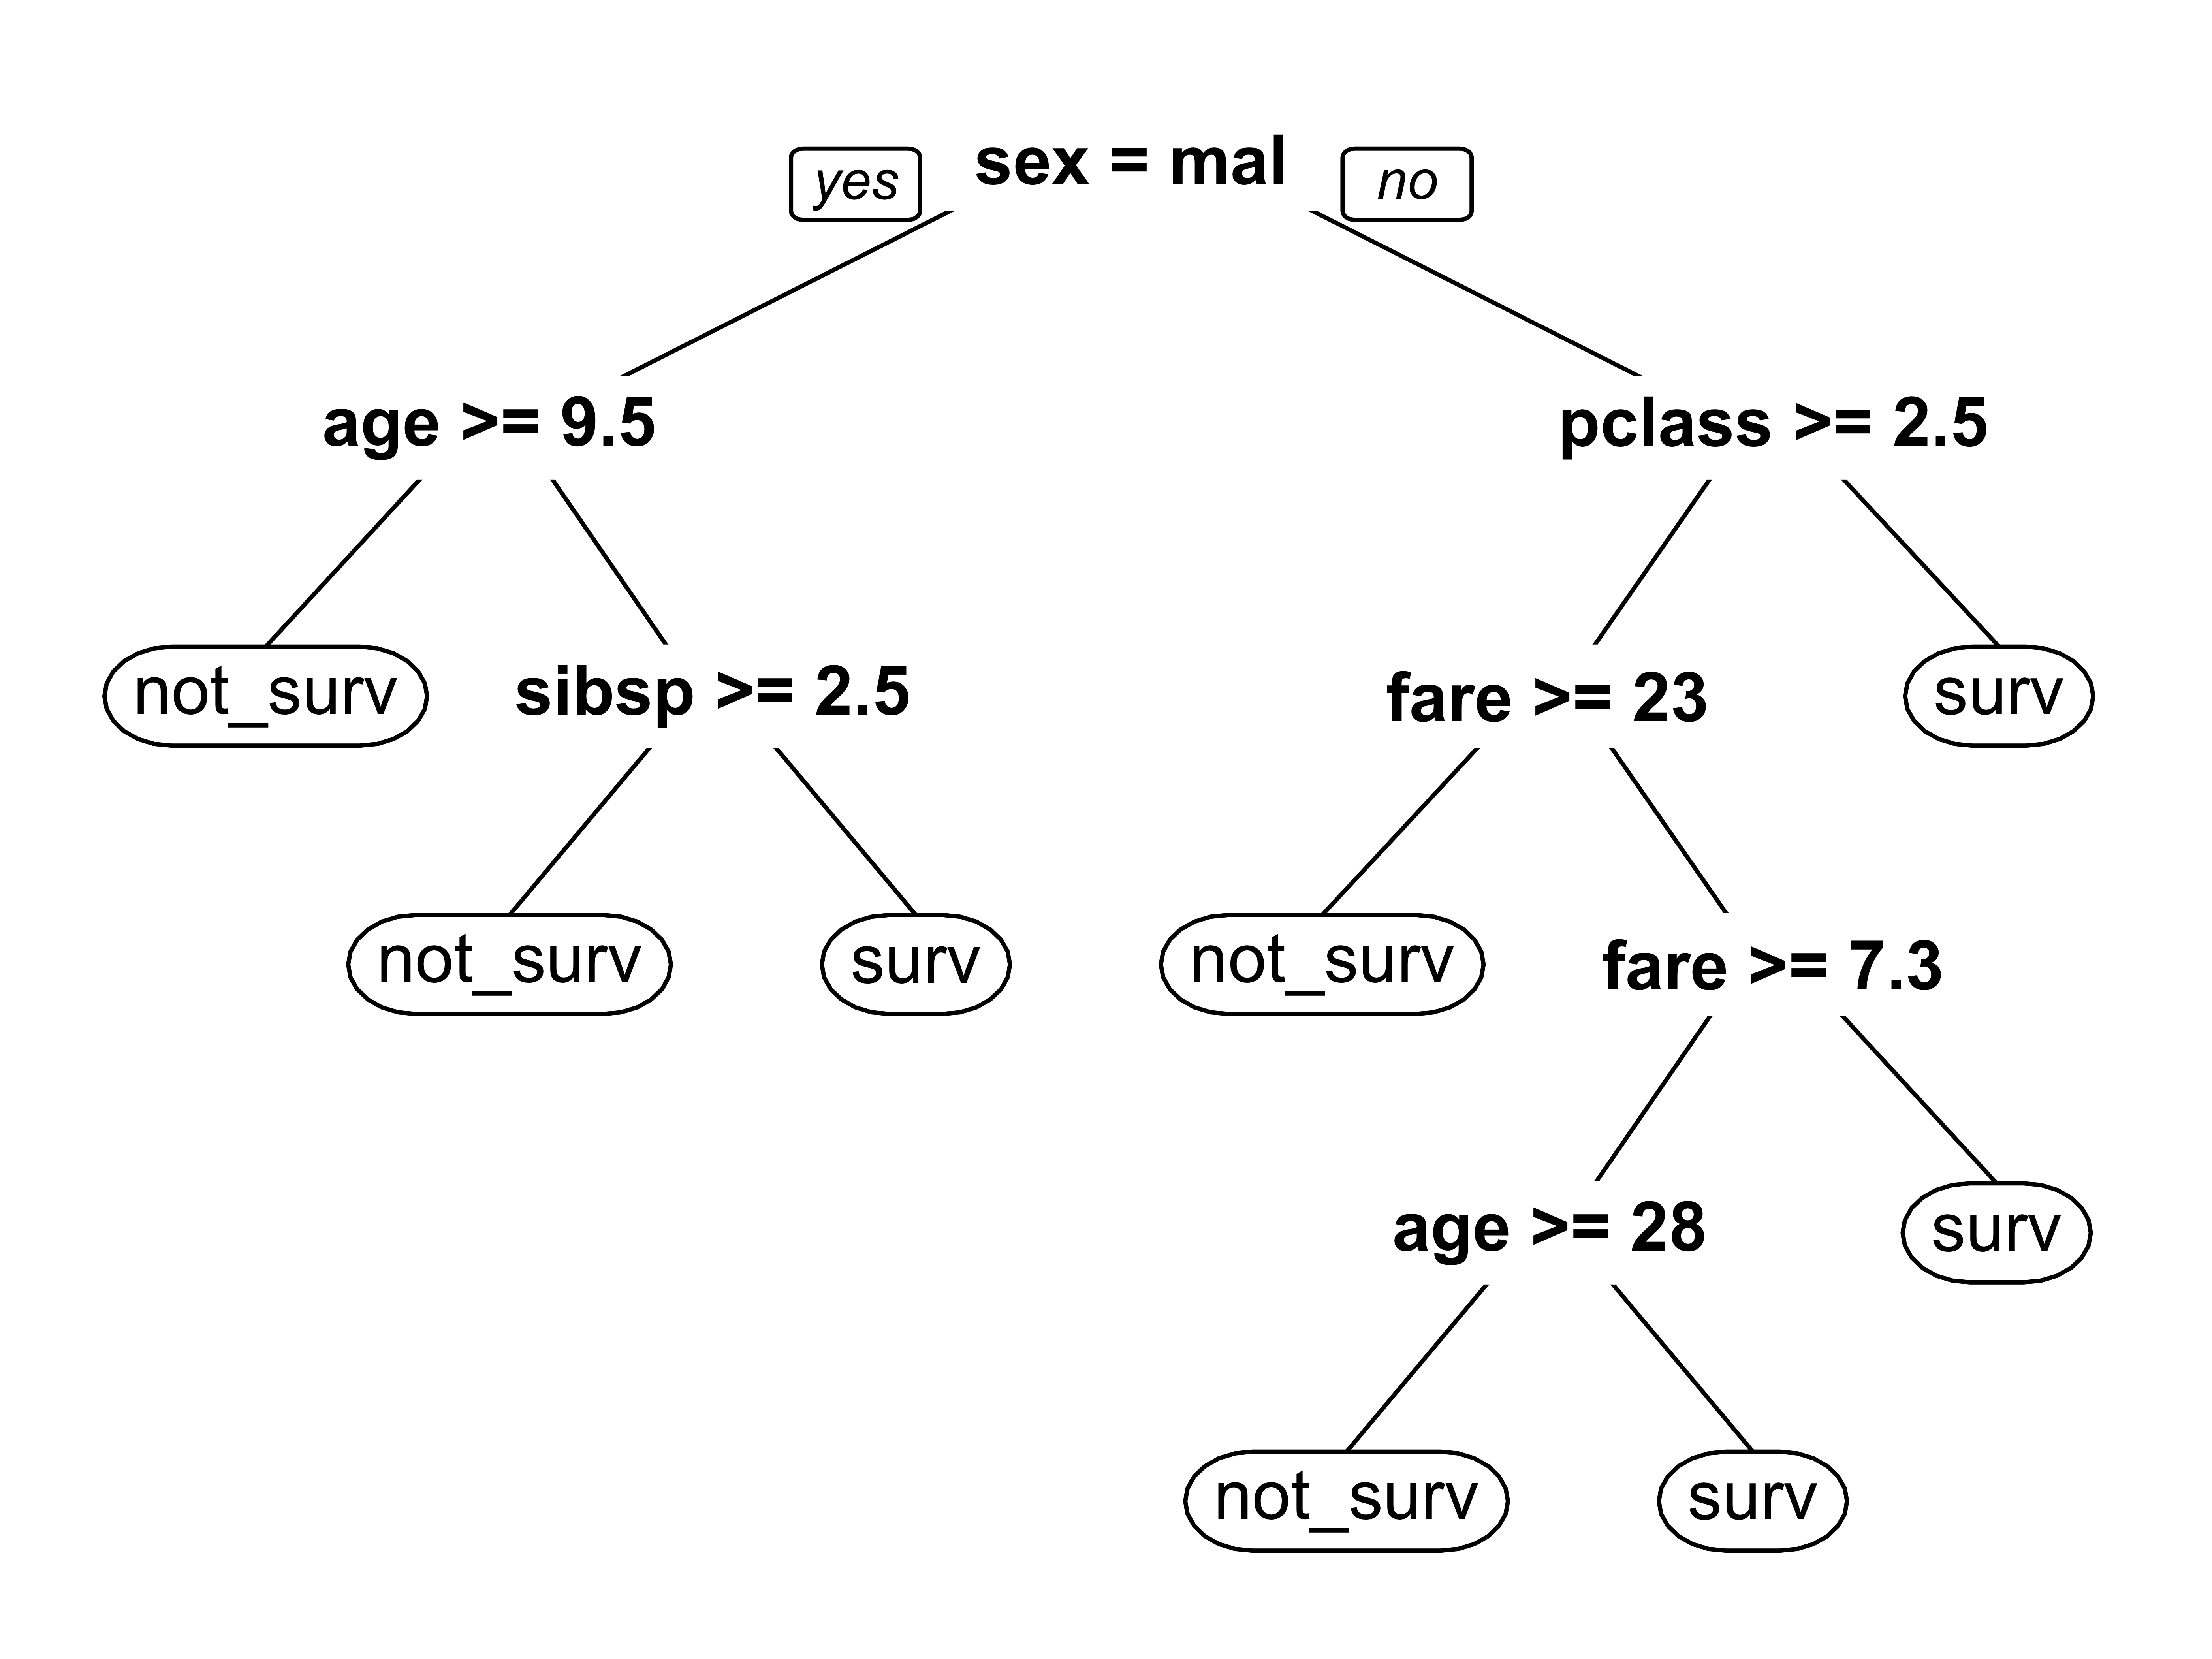
\includegraphics[scale = 0.05]{/Users/payforsoup/Documents/Non-School/Talks/SEI/tree.png}
			\end{figure}		
    		\end{frame}

	
	\subsection{CART}
	
		\begin{frame}{Classification and Regression Trees}
			\begin{enumerate}
				\item{Breiman, Friedman, Olshen, \& Stone (1984)}
				\item{Tree built by recursive binary splits}
				\item{Splits determined by minimizing node impurity \\}
				\begin{center}
					$$\sum_{k = 1}^{K} \hat{p}_{mk}(1 - \hat{p}_{mk})$$
				\end{center}
				where \\
				\begin{center}
					$$ \hat{p}_{mk} = \frac{1}{N_m} \sum_{x_i \in R_m} I(y_i = k)$$
				\end{center}
				is proportion of class $k$ observations in node $m$		
			\end{enumerate}
		\end{frame}
		
		\begin{frame}{Advantages of Trees-Based Models}
			\begin{enumerate}
				\item{Intuitive}
				\item{Handle interactions naturally}
				\item{Minimal assumptions}
			\end{enumerate}
		\end{frame}
	
	
	\subsection{Disadvantages of Trees}
		
		\begin{frame}{Disadvantages of Single Trees}
			\begin{enumerate}
				\item{Prone to overfitting}
				\item{Tree does well with original sample, but accuracy suffers with new data}
			\end{enumerate}
		\end{frame}
		
\subsection{Bagging}
		\begin{frame}{Bootstrap Aggregation (Bagging)}
			\begin{enumerate}
				\item{Breiman (1996)}
				\item{Extends idea of CART models}
					\begin{enumerate}[1]
						\item{Single trees overfit}
						\item{Stopping rules and pruning help, but only to a point}
					\end{enumerate}
				\item{Take many bootstrap samples, build many trees, aggregate predictions}
			\end{enumerate}
    		\end{frame}
	
		\begin{frame}{Bootstrap Samples}
		$x := [1.9, 2.4, 3.2, 1.7, 0.3]$
		\begin{table}
		\begin{tabular}{c c c}
			\hline
			$B^{*1}$	& $B^{*2}$& $B^{*3}$  \\
			\hline
			0.3 		& 2.4 	& 2.4  \\
			1.9 		& 1.7 	& 0.3 \\
			1.9		& 0.3		& 2.4 \\
			2.4 		& 0.3 	& 2.4 \\
			1.9		& 1.9		& 0.3 \\
			\hline
		\end{tabular}
		\end{table}
		\end{frame}
		
		
		\begin{frame}{Bagging Pseudocode}
			\begin{enumerate}[]
				{\fontfamily{cmr}\selectfont
				\item{\textbf{for} $i = 1:B$}
					\begin{enumerate}[]
						\item{\hspace{3 mm} Sample random $N$ records with replacement}
						\item{\hspace{3 mm} Fit classification tree}
						\item{\hspace{3 mm} Add $i^{th}$ tree to ensemble}
					\end{enumerate}
				\item{\textbf{endfor}}
				\item{Aggregate predictions for input $\textbf{X}$}
				}
			\end{enumerate}
		\end{frame}
	
		
		\begin{frame}{Advantages of Bagging}
			\begin{enumerate}
				\item{Big improvement in predictive performance}
				\item{Variance decreases}
				\item{Easy to tune}
				\item{Out-of-bag (OOB) error estimate}
			\end{enumerate}
		\end{frame}

		
	
	\subsection{RF}
		\begin{frame}{Random Forests}
    			\begin{enumerate}
				\item{Ho (1995), Breiman (2001)}
				\item{Extends idea of bagging}
				\item{Build many trees, aggregate predictions}
				\item{Only consider $m$ predictors at each node}
				\item{Improve predictive performance}
					\begin{enumerate}[1]
						\item{Reduce inter-tree correlation}
						\item{Further reduce variance beyond bagging}
					\end{enumerate}
			\end{enumerate}
    		\end{frame}


\section{Ensemble Methods}
	\subsection{Why Ensemble Methods?}
	
		\begin{frame}{Ensemble Concept}
			\begin{enumerate}
				\item{Fit many simple models, then aggregate}
				\item{Result is ``committee'' of learners}
				\item{In classification problems, each casts a vote}
				\item{Examples}
				\begin{enumerate}[1]
					\item{Boosting}
					\item{Bagging}
					\item{Random forests}
				\end{enumerate}
			\end{enumerate}
		\end{frame}
				
		
		\begin{frame}{Advantages of Ensemble Methods}
			\begin{enumerate}
				\item{Hugely powerful prediction models}
				\item{Usually have few meta-parameters to tune}
				\item{Very powerful ``off-the-shelf''}
				\item{Interpretability (\textit{contra} neural networks)}
			\end{enumerate}
		\end{frame}
	
	
	
	
		\begin{frame}{Random Forest Pseudocode}
			\begin{enumerate}[]
				{\fontfamily{cmr}\selectfont
				\item{\textbf{for} $i = 1:B$}
					\begin{enumerate}[  ]
						\item{\hspace{3 mm} Sample random $N$ records with replacement}
						\item{\hspace{3 mm} Select $m$ predictors from complete set of $p$ predictors}
						\item{\hspace{3 mm} Fit classification tree, using only $m$ predictors}
						\item{\hspace{3 mm} Add $i^{th}$ tree to ensemble}
					\end{enumerate}
				\item{\textbf{endfor}}
				\item{Aggregate predictions for input $\textbf{X}$}
				}
			\end{enumerate}
		\end{frame}
	

		\begin{frame}{Advantages of Random Forests}
			\begin{enumerate}
				\item{Powerful prediction models}
				\item{Easy to tune}
				\item{Will not overfit}
				\item{Variable importance}
				\item{Out-of-bag (OOB) error estimate}
			\end{enumerate}
		\end{frame}




\section{Analysis}
	
		
	\subsection{Conclusion}	
		
		\begin{frame}{\hspace{3 mm}}
			\begin{center}
			Thank you!
			\end{center}
		\end{frame} 
		
		
		
\end{document}